\section{Answers to Assignment Questions}

\noindent \textbf{Q1. After DROPping echo-reply packets on OUTPUT chain, what 
was the observed effect? Use Figure~\ref{fig:icmpexample} to illustrate the 
path of the packets. Mark the path with arrows and use an X to mark the point 
where the packets are DROPped.}
~\ \\

\noindent \textbf{Q2. After DROPing echo-request packets on INPUT chain, what
was the observed effect? How is this reaction different from the reaction
achieved in Q1? Use Figure~\ref{fig:icmpexample} to illustrate the path of 
the
packets. Mark the path with arrows and use an X to mark the point where the
packets are DROPped.}
~\ \\

\begin{figure}[!ht]
    \begin{center}
        \subfigure[Use this Figure to explain Q1]{
            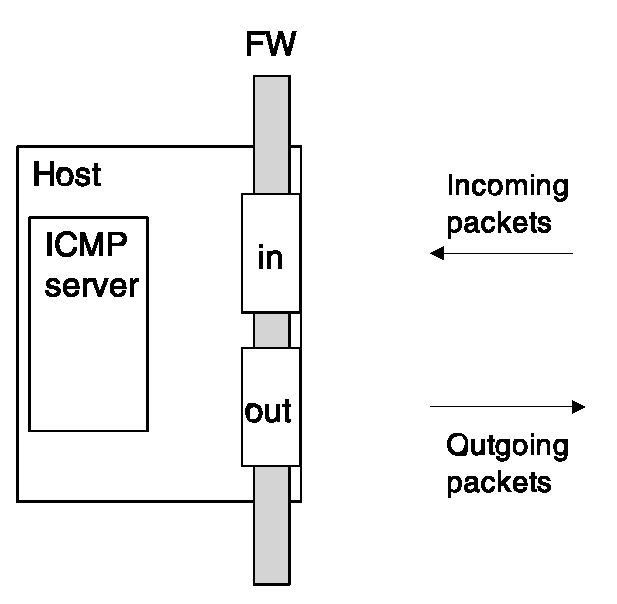
\includegraphics[scale=0.5]{figures/icmpexample.eps}
            \label{fig:icmpexampleQ1}
        }
        \hspace{1in}
        \subfigure[Use this Figure to explain Q2]{
            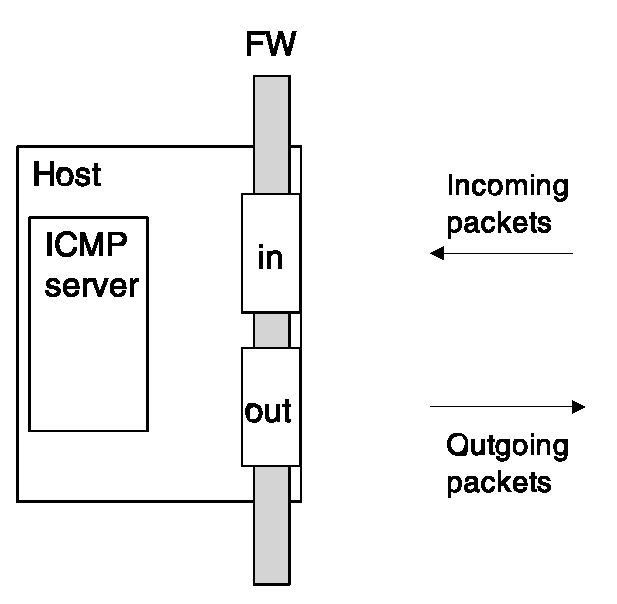
\includegraphics[scale=0.5]{figures/icmpexample.eps}
            \label{fig:icmpexampleQ2}
        }
    \end{center}
    \caption{Figure to help you illustrate your thoughts regarding the packet 
        flow in questions Q1 and Q2.}
    \label{fig:icmpexample}
\end{figure}

\noindent \textbf{Q3. For each entry in the log, several information items are
displayed. Some entries can be useful for creating new rules. Explain the 
items \texttt{IN}, \texttt{OUT}, \texttt{SRC}, \texttt{DST} and \texttt{PROTO}
mean and why these might be useful.}
~\ \\

\noindent \textbf{Q4. At this stage, with default policy set to DROP for all 
chains, would you consider the system secure? Would you consider it useful?}
~\ \\

\noindent \textbf{Q5. Assume instead that you used default policy ACCEPT, 
would you consider the system secure now? Would you consider it useful?}
~\ \\

\noindent \textbf{Q6. You just added some protection against flooding by 
limiting the number of packets the firewall will let through to 1 per second. 
Give two examples on how you can tell that you are protected!}
~\ \\
